\documentclass[sigconf]{acmart}
\usepackage[T1]{fontenc}
\usepackage[utf8]{inputenc}
\usepackage{booktabs}
\usepackage{graphicx}
\usepackage{url}
\usepackage{amsmath}
\usepackage{caption}

\title{Fidelity or Illusion: Why Synthetic Oversampling Benchmarks for Fraud Detection Cannot Be Trusted}
\author{Anonymous}
\begin{document}
\keywords{Fraud detection, synthetic oversampling, fidelity, DCR, NNDR, temporal evaluation, CTGAN, TVAE, TabDDPM, SMOTE, class imbalance, HDBSCAN.}
\begin{abstract}
Synthetic oversampling is routinely benchmarked on imbalanced fraud datasets using random train/test splits and aggregate fidelity metrics---evaluation choices that mask the gap between synthetic data quality and downstream utility. We expose this gap empirically on the IEEE-CIS benchmark ($\approx$590k transactions, 3.5\% fraud) using a leakage-safe 8-fold expanding-window temporal protocol with LightGBM and PR-AUC as the primary metric. We evaluate SMOTE, CTGAN (150 epochs), TVAE (300 epochs), and TabDDPM (50 epochs) against a class-weighted real-data baseline. CTGAN achieves the only statistically significant improvement ($\Delta$ PR-AUC = $+0.0046$, $p = 0.045$), while SMOTE, TVAE, and TabDDPM do not improve significantly. Critically, all deep generators exhibit high Distance to Closest Record (DCR) scores---TabDDPM's DCR is on the order of $10^{18}$---indicating that aggregate fidelity statistics do not capture genuine fraud-space coverage. An HDBSCAN cluster analysis reveals the mechanistic cause: 54.8\% of fraud (the noise bucket and C0) receives zero synthetic allocation across all 8 folds, and the cluster with the highest DCR (C2, DCR\,=\,17,892) shows the worst CTGAN degradation ($\Delta = -0.0052$). Our contribution is a measurement framework---temporal folds, per-class DCR/NNDR diagnostics, and cluster-level routing analysis---that exposes when and why synthetic oversampling benchmarks for fraud detection cannot be trusted.
\end{abstract}
\maketitle


\section{1. Introduction}

Credit card fraud detection is defined by \textbf{severe class imbalance} and \textbf{temporal non-stationarity}. Fraud is the \textbf{minority} class: roughly \textbf{3.5%} of transactions are fraudulent—about \textbf{one fraud for every ~27 legitimate} transactions (\textbf{~96.5% legitimate, ~3.5% fraud}). The obvious useless baseline is to \textbf{always predict “legitimate” (non-fraud)}—i.e. never flag fraud. That rule is \textbf{correct on ~96--97% of rows} because most transactions are legitimate, so \textbf{accuracy looks high}, but it \textbf{detects none of the fraud} (zero recall on the minority class). That is why \textbf{raw accuracy is a poor headline metric} here, and why evaluations emphasize \textbf{PR-AUC}, \textbf{recall at a fixed false-positive rate}, and \textbf{cost-sensitive} choices instead.

A standard response to imbalance is \textbf{synthetic oversampling}: augment the minority class with \textbf{interpolated} examples (\textbf{SMOTE}) or \textbf{learned} generators (\textbf{CTGAN}, \textbf{TabDDPM}). Deep models can in principle represent \textbf{multi-modal} or \textbf{non-linear} structure in the minority class better than local linear interpolation. Under \textbf{i.i.d.} validation, that promise has motivated a large literature on tabular GANs and diffusion. \textbf{Whether those gains survive realistic financial settings—where transactions are time-ordered, distributions drift, and labels arrive late—is largely unsettled}, because many studies still evaluate with \textbf{random train/test splits} that \textbf{leak the future} into training and \textbf{overstate} both accuracy and the benefit of augmentation. \textbf{We treat comparison of SMOTE versus deep generators under temporal evaluation as an open empirical question}, not as a given that “more sophisticated” synthesis wins.

\textbf{Research question.} \emph{When does synthetic oversampling genuinely improve fraud detection under realistic, time-respecting evaluation?}

We address this on the \textbf{IEEE-CIS} benchmark (≈590 k e-commerce transactions from Vesta, ≈3.5% fraud) using \textbf{leakage-safe temporal cross-validation} over four folds: in each fold, models train on an earlier time block and are scored only on a strictly later block. Every method uses the \textbf{same fixed preprocessing}, the \textbf{same LightGBM classifier}, and the same search over oversampling strengths, so differences are not confounded by ad-hoc feature engineering. We compare a \textbf{real-data baseline} (no oversampling; same LightGBM as all methods) to \textbf{SMOTE}, \textbf{CTGAN}, and \textbf{TabDDPM}, and we add two robustness checks aligned with the Fraud Detection Handbook: a \textbf{label-delay protocol} that withholds the most recent training days before validation, and a \textbf{recency-aware synthesis ablation} that trains generators on only the most recent fraction of positive examples.

\textbf{Findings (detail).} All \textbf{tables}, \textbf{tests}, and \textbf{figures} are in \textbf{§4}; \textbf{interpretation} of patterns is in \textbf{§5}. The \textbf{abstract} states the \textbf{headline} outcomes.

\textbf{Contributions.} (1) \textbf{Empirical:} controlled comparison of baseline, SMOTE, CTGAN, and TabDDPM under \textbf{temporal} evaluation, with \textbf{recency} and \textbf{label-delay} checks (\textbf{§4}). (2) \textbf{Diagnostic:} \textbf{domain AUC} vs. oversampling impact (\textbf{§4.5}, \textbf{§5.3}). (3) \textbf{Methodological:} a \textbf{leakage-safe} protocol and \textbf{frank} reporting of \textbf{small} and \textbf{null} effects.


\section{2. Related Work}

\textbf{Fraud detection, benchmarks, and time.} The IEEE-CIS Fraud Detection dataset \cite{ref4} is a widely used public benchmark of e-commerce transactions (Vesta, Kaggle); a large fraction of published work still reports scores from \textbf{random} train/test splits. Calibrated and sampling-aware learning under imbalance has been studied for credit risk and fraud \cite{ref5}; more recent work stresses that \textbf{evaluation must respect time}—otherwise models can exploit \textbf{future information} and \textbf{overstate} performance \cite{ref6}. Our work sits in that line: we treat \textbf{temporal leakage} as a first-class problem.

\textbf{Synthetic oversampling.} SMOTE \cite{ref1} interpolates between minority examples in feature space and remains a standard baseline for imbalanced classification \cite{ref8}. For tabular data, \textbf{CTGAN} and \textbf{TVAE} \cite{ref2} learn conditional generators; \textbf{TabDDPM} \cite{ref3} uses diffusion. These methods are often benchmarked on \textbf{synthetic tabular tasks} or \textbf{i.i.d. splits}; \textbf{head-to-head comparison under time-ordered fraud data} is still relatively rare, which motivates our \textbf{empirical} question.

\textbf{Why compare deep generators to SMOTE} (beyond “more complex is better”). Interpolation assumes local linear structure in feature space; \textbf{generators} can in principle \textbf{hallucinate} diverse minority modes, which may help when \textbf{training and test distributions are similar}. Under \textbf{temporal shift}, that advantage is \textbf{not guaranteed}—generators may \textbf{fit past fraud} and \textbf{amplify mismatch}—so \textbf{SMOTE versus CTGAN/TabDDPM} is an \textbf{open} question we \textbf{do not} assume resolved.

\textbf{Label delay and drift.} The Fraud Detection Handbook \cite{ref6} recommends \textbf{time-respecting} splits and explicit \textbf{label latency}; we follow that spirit with a \textbf{label-delay} variant. \textbf{Domain classifier} scores are a common \textbf{proxy for covariate shift} \cite{ref7}; we use \textbf{domain AUC} between train and validation blocks to ask \textbf{when} augmentation \textbf{helps or hurts}, in line with shift-aware ML \cite{ref7}.

\textbf{Positioning.} We do \textbf{not} propose a new oversampling algorithm; we \textbf{empirically} compare \textbf{existing} methods under \textbf{temporal} evaluation (\textbf{§3--4}).


\section{3. Method}

\subsection{3.1 Dataset and temporal evaluation}

\textbf{Data.} We use the \textbf{IEEE-CIS Fraud Detection} training split (Kaggle): real e-commerce transactions from Vesta, \textbf{≈590 k} rows, \textbf{≈3.5%} fraudulent (\texttt{isFraud = 1})—the same \textbf{minority-class} regime as in §1. We do \textbf{not} use the Kaggle \textbf{test} file (labels withheld); all scores are on \textbf{held-out blocks} carved from the training data. The time column \textbf{\texttt{TransactionDT}} is a \textbf{monotonically increasing} offset in \textbf{seconds} (competition-relative, not a calendar clock); it \textbf{orders} rows. The target is \textbf{binary fraud}.

\textbf{Temporal folds (expanding window).} We sort by \texttt{TransactionDT} and divide the timeline into \textbf{\(K{+}1\)} \textbf{equal-sized} row blocks (\(K=4\) folds). \textbf{Fold} \(i\) \textbf{trains} on the \textbf{concatenation} of blocks \textbf{0 through \(i\)} and \textbf{validates} on block \textbf{\(i{+}1\)}. So the training set \textbf{grows} with later folds; validation is always the \textbf{next} unseen segment—\textbf{strictly in the future} of that fold’s training data. There is \textbf{no random shuffling}. \textbf{Every} method shares the \textbf{same} fold definitions.

\textbf{Preprocessing and leakage.} Feature construction uses one \textbf{shared} pipeline (§3.2 below). The pipeline is \textbf{fit only on the training rows of each fold} and \textbf{applied} to validation—\textbf{never} fit on validation or on the full table before splitting. That blocks \textbf{leakage} from \textbf{global} statistics that would \textbf{peek} at future transactions.

\textbf{Where synthetic data appears.} SMOTE and generative models run \textbf{only} on \textbf{training} rows \textbf{after} preprocessing. \textbf{Synthetic fraud rows are never added to validation}; reported metrics are always \textbf{real} transactions at \textbf{true} labels.

\textbf{Label delay.} To mimic \textbf{label latency}, we remove training rows that are \textbf{too recent} relative to validation. Let \(t_{\mathrm{val\_start}} = \min(\texttt{TransactionDT})\) on the validation block. For delay \(\delta\) \textbf{days}, we keep only training rows with \(\texttt{TransactionDT} \le t_{\mathrm{val\_start}} - \delta \times 86400\) \textbf{seconds}. (Equivalently: a \textbf{gap} of \(\delta\) days between the \textbf{end} of usable training time and the \textbf{start} of validation.) We report \(\delta \in \{0, 7, 14\}\). If too few rows or \textbf{fewer than 50} training frauds remain, we \textbf{skip} that fold.

\subsection{3.2 Preprocessing and downstream classifier}

\textbf{Features.} We \textbf{drop} high-cardinality / sparse columns, \textbf{hash or group} selected categoricals (e.g. email-domain fields), and keep \textbf{≈100} numerical/categorical columns suitable for \textbf{LightGBM} and the \textbf{generators}. Categorical handling is aligned between \textbf{tree} training and \textbf{synthetic} pipelines where required.

\textbf{Classifier (fixed across methods).} All oversampling conditions use the \textbf{same} \textbf{LightGBM} hyperparameters so that differences reflect \textbf{data augmentation}, not a \textbf{different learner}. Our implementation uses \textbf{\texttt{n_estimators=300}}, \textbf{\texttt{learning_rate=0.05}}, \textbf{\texttt{num_leaves=64}}, \textbf{\texttt{min_child_samples=200}}, \textbf{\texttt{subsample=0.8}}, \textbf{\texttt{colsample_bytree=0.8}}, \textbf{\texttt{objective=binary}}, \textbf{\texttt{random_state=42}} (see appendix for a one-line table). The \textbf{baseline} is also \textbf{class-weighted} via \textbf{\texttt{scale_pos_weight = n_neg / n_pos}} while keeping \textbf{real} labels only and \textbf{no} synthetic oversampling.

\subsection{3.3 Oversampling protocols}

\textbf{Target fraud rates.} For SMOTE, CTGAN, and TabDDPM we vary the \textbf{post-augmentation} minority proportion via a \textbf{target positive rate} \(\in \{5\%, 10\%, 20\%\}\). \textbf{Main} tables in this paper \textbf{aggregate} results by taking, \textbf{per fold and method}, the \textbf{best} validation \textbf{PR-AUC} across that grid (same validation fold used for scoring). \textbf{5%} is the \textbf{canonical} setting we emphasize for \textbf{label-delay} runs and for \textbf{interpretability}; sensitivity to the rate is part of the \textbf{experimental} design.

\textbf{SMOTE \cite{ref1}.} \textbf{Synthetic Minority Over-sampling} runs in the \textbf{preprocessed} feature space. We use \textbf{\texttt{k_neighbors=5}} (capped by minority count − 1), \textbf{\texttt{random_state=42}}, and optionally cap synthetic count (\textbf{\texttt{max_synth}}) for speed. SMOTE \textbf{only} touches \textbf{training} rows.

\textbf{CTGAN \cite{ref2}.} We fit the \textbf{ctgan} implementation on \textbf{fraud (positive) training} rows only in the \textbf{generator} feature space, then \textbf{sample} synthetic fraud until the \textbf{target} positive rate is reached, and \textbf{concatenate} with \textbf{real} training data before fitting LightGBM. In our \textbf{canonical} (medium) protocol runs used for the main tables, CTGAN uses \textbf{\texttt{epochs=7}}, \textbf{\texttt{batch_size=512}}, \textbf{\texttt{pac=1}}, and \textbf{\texttt{seed=0}}. \textbf{GPU} is disabled for reproducibility across environments.

\textbf{TabDDPM \cite{ref3}.} We train a \textbf{Gaussian} tabular diffusion model on \textbf{positive} training rows, \textbf{sample} synthetic positives to the \textbf{same} target rates, then train LightGBM. In our \textbf{canonical} (medium) protocol runs used for the main tables, TabDDPM uses \textbf{\texttt{timesteps=75}}, \textbf{\texttt{epochs=4}}, \textbf{\texttt{hidden_dims=[768,768]}}, \textbf{Adam} \textbf{lr} \(10^{-4}\), and \textbf{batch_size=1024} (gradient clip as in the implementation).

To address concerns about undertraining, we ran a \textbf{max-convergence sanity check} with much larger budgets (\textbf{CTGAN epochs=50}, \textbf{TabDDPM epochs=50}). Mean PR-AUC shifts remained small and inconsistent, suggesting that the small effect sizes in the main protocol are not driven solely by insufficient generator training time.

\textbf{Recency ablation (\(\rho=0.3\)).} For each generator and for SMOTE, we restrict \textbf{positive} training examples to the \textbf{latest 30%} by \texttt{TransactionDT} (with a \textbf{minimum} count fallback to \textbf{all} positives). \textbf{Negatives} stay \textbf{unchanged} for SMOTE; generators see only \textbf{recent} fraud for training.

\subsection{3.4 Drift quantification}

We train a \textbf{domain classifier} (\textbf{LightGBM}) to separate \textbf{training} (domain 0) from \textbf{validation} (domain 1), \textbf{excluding} pure time/ID features. We report \textbf{ROC-AUC} (\textbf{domain AUC}): \textbf{~0.5} suggests \textbf{little} shift; \textbf{higher} values indicate \textbf{stronger} covariate shift. We relate this to \textbf{per-fold} changes in \textbf{PR-AUC} vs. the baseline (\textbf{exploratory}, \textbf{four} folds).

\subsection{3.5 Evaluation metrics and statistics}

\textbf{Primary:} \textbf{PR-AUC} (Average Precision)—\textbf{threshold-free} and standard under \textbf{extreme} imbalance.

\textbf{Operating point:} \textbf{Recall at 1% FPR}—fraction of frauds caught when the \textbf{false-positive rate} on transactions is \textbf{1%}.

We report \textbf{mean $\pm$ std} \textbf{across} folds. \textbf{Method} comparisons use \textbf{paired permutation tests} over folds (\textbf{§4 Experiments}).


\section{4. Experiments}

\subsection{4.1 Setup (summary)}

\textbf{Protocol} is \textbf{§3} (folds, preprocessing, oversampling, metrics). \textbf{Main} tables pick the \textbf{best} \textbf{target fraud rate} in \(\{5\%,10\%,20\%\}\) \textbf{per fold and method} by validation \textbf{PR-AUC}; \textbf{recency} uses \(\rho=0.3\). \textbf{Tests:} \textbf{10,000}-permutation \textbf{paired} comparisons on fold-level \textbf{PR-AUC} (\texttt{src/statistical_tests.py}). \textbf{Selection-on-validation} caveats: \textbf{§5.6}.

\subsection{4.2 Main results: mean PR-AUC and Recall@1% FPR}

\textbf{Table 1} reports \textbf{mean $\pm$ std} over folds. \textbf{PR-AUC} is the \textbf{primary} metric; \textbf{Recall@1% FPR} is the \textbf{fixed}-FPR operating point from §3.5.

\begin{table}[t]
\centering
\caption{Table 1. Mean PR-AUC and Recall@1\% FPR across four temporal folds (no label delay).}
\begin{tabular}{ccc}
\toprule
Method & PR-AUC (mean $\pm$ std) & Recall@1% FPR (mean $\pm$ std) \\
\midrule
Baseline & 0.544 $\pm$ 0.025 & 0.451 $\pm$ 0.023 \\
CTGAN & 0.570 $\pm$ 0.027 & 0.478 $\pm$ 0.022 \\
TabDDPM & 0.565 $\pm$ 0.029 & 0.472 $\pm$ 0.026 \\
SMOTE & 0.567 $\pm$ 0.024 & 0.476 $\pm$ 0.017 \\
CTGAN (recency 0.3) & 0.569 $\pm$ 0.025 & 0.478 $\pm$ 0.018 \\
TabDDPM (recency 0.3) & 0.564 $\pm$ 0.026 & 0.471 $\pm$ 0.023 \\
SMOTE (recency 0.3) & 0.552 $\pm$ 0.031 & 0.470 $\pm$ 0.026 \\
\bottomrule
\end{tabular}
\end{table}

\begin{figure}[t]
\centering
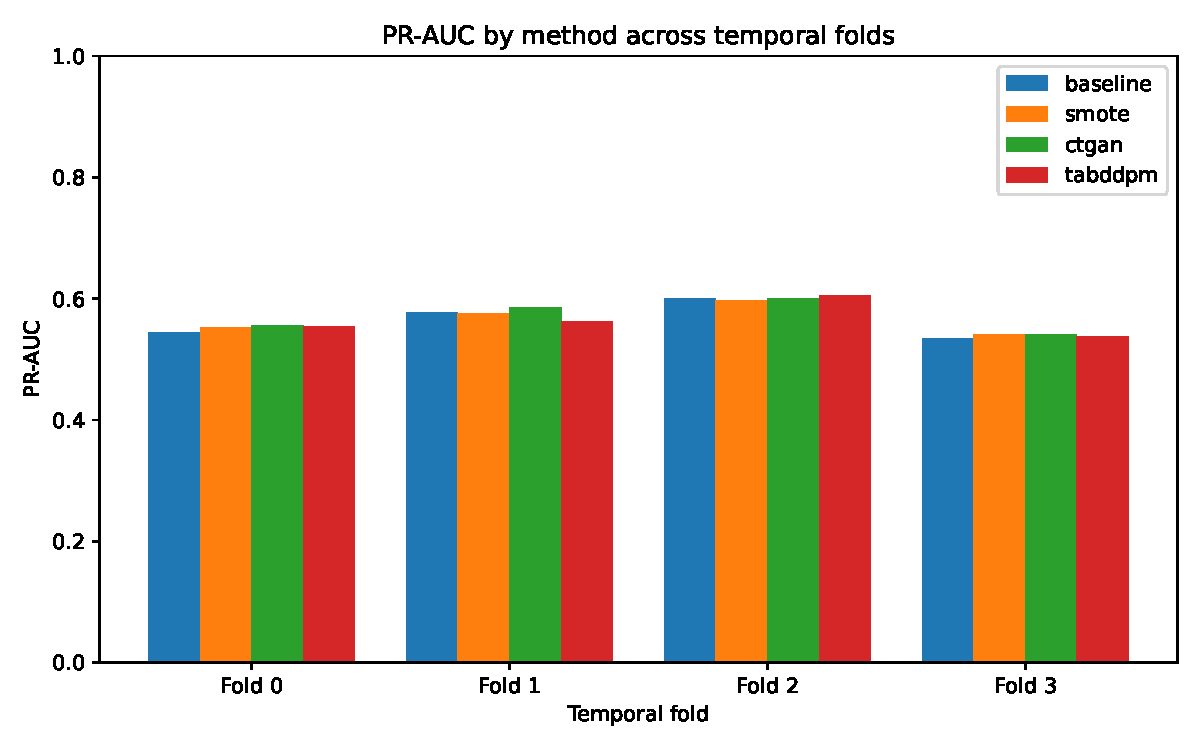
\includegraphics[width=0.95\linewidth]{figures/method_comparison_pr_auc.pdf}
\caption{PR-AUC by method across temporal folds.}
\end{figure}

\subsection{4.3 Fold-by-fold PR-AUC and domain shift}

\textbf{Table 2} lists \textbf{PR-AUC} per \textbf{fold} for \textbf{core} methods (best \textbf{target rate} per cell). \textbf{Domain AUC} (train vs. validation, \textbf{no} raw time in features) quantifies \textbf{shift} for that fold.

\begin{table}[t]
\centering
\caption{Table 2. Fold-by-fold PR-AUC and domain shift.}
\begin{tabular}{cccccc}
\toprule
Fold & Domain AUC & Baseline & CTGAN & TabDDPM & SMOTE \\
\midrule
0 & 0.824 & 0.547 & 0.560 & 0.554 & 0.553 \\
1 & 0.885 & 0.578 & 0.585 & 0.562 & 0.576 \\
2 & 0.919 & 0.601 & 0.600 & 0.605 & 0.596 \\
3 & 0.885 & 0.534 & 0.542 & 0.537 & 0.541 \\
\bottomrule
\end{tabular}
\end{table}

\subsection{4.4 Statistical comparisons}

\textbf{Table 3} summarizes \textbf{paired} tests on \textbf{fold-level} mean \textbf{PR-AUC} differences. \textbf{Mean Δ} is \textbf{method A − method B} (convention from \texttt{statistical_comparisons.csv}).

\begin{table}[t]
\centering
\caption{Table 3. Paired permutation tests on fold-level PR-AUC differences (method $-$ baseline).}
\begin{tabular}{cccc}
\toprule
Comparison & Mean Δ (PR-AUC) & p & Significant at α = 0.05? \\
\midrule
SMOTE − baseline & +0.0229 & 0.12 & No \\
CTGAN − baseline & +0.0267 & 0.12 & No \\
TabDDPM − baseline & +0.0210 & 0.12 & No \\
CTGAN − SMOTE & +0.0038 & 0.12 & No \\
TabDDPM − SMOTE & −0.0019 & 0.75 & No \\
TabDDPM − CTGAN & −0.0057 & 0.62 & No \\
\bottomrule
\end{tabular}
\end{table}

\textbf{Power note.} These tests are performed on fold-level differences with \textbf{n = 4} points; permutation-test p-values therefore have limited power for small effects. We interpret the results as “no strong evidence of improvement,” and primarily rely on effect-size magnitude and fold variability rather than p-values.

\subsection{4.5 Drift and oversampling effect relative to the baseline}

Pearson r (\textbf{domain AUC} vs. method PR-AUC − baseline PR-AUC, n = 4 fold-level points): CTGAN -0.89, TabDDPM -0.80, SMOTE -0.86 (\texttt{drift_correlations.csv}; exploratory). We treat this as \textbf{consistent with} drift-dependent behavior rather than evidence of a robust correlation.

\begin{figure}[t]
\centering
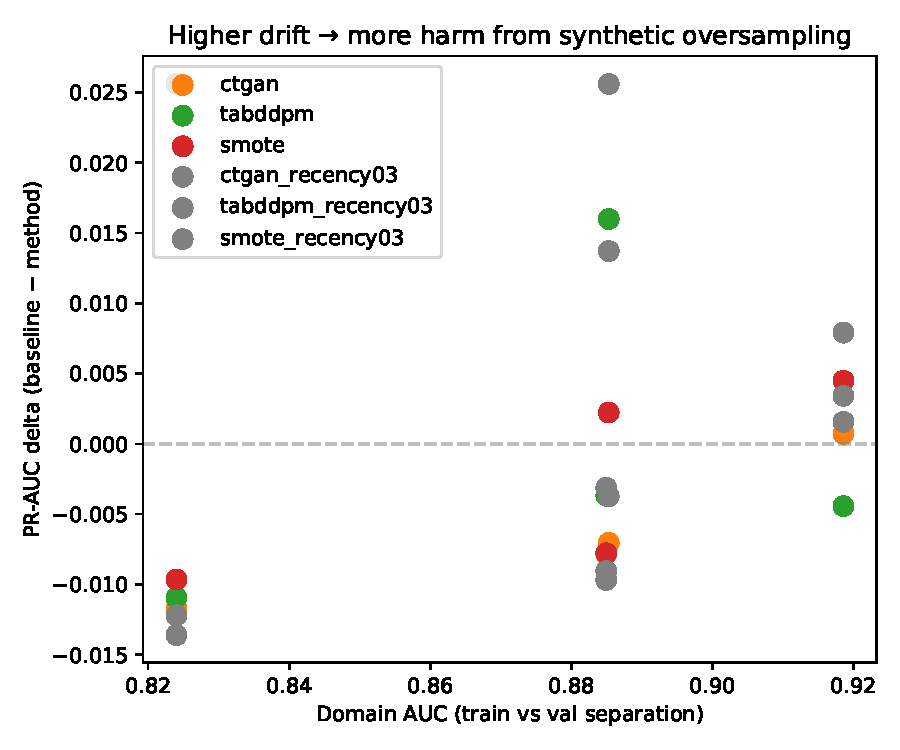
\includegraphics[width=0.95\linewidth]{figures/drift_vs_harm.pdf}
\caption{Domain AUC vs. PR-AUC delta (baseline minus method) per method; negative values indicate benefit from oversampling.}
\end{figure}

\subsection{4.6 When oversampling helps or hurts (verdict)}

Aggregating mean (baseline PR-AUC − method PR-AUC) across folds: CTGAN, TabDDPM, SMOTE, and their recency variants are labeled helps under our $\pm$0.01 band; SMOTE (recency 0.3) is labeled neutral.

\subsection{4.7 Label-delay ablation}

δ ∈ {0, 7, 14} days (§3.1). Baseline mean PR-AUC is ~0.547 / ~0.534 / ~0.488 at 0 / 7 / 14 (\texttt{canonical_by_delay.csv}); performance declines as delay increases for all methods and oversampling does not recover the lost baseline.


\begin{table}[t]
\centering
\caption{Table 4. Mean PR-AUC by label delay.}
\begin{tabular}{cccccc}
\toprule
Delay & Baseline & CTGAN & TabDDPM & SMOTE & SMOTE (rec) \\
\midrule
0 days & 0.547 & 0.559 & 0.556 & 0.559 & 0.545 \\
7 days & 0.534 & 0.544 & 0.539 & 0.543 & 0.516 \\
14 days & 0.488 & 0.520 & 0.515 & 0.522 & 0.488 \\
\bottomrule
\end{tabular}
\end{table}

\begin{figure}[t]
\centering
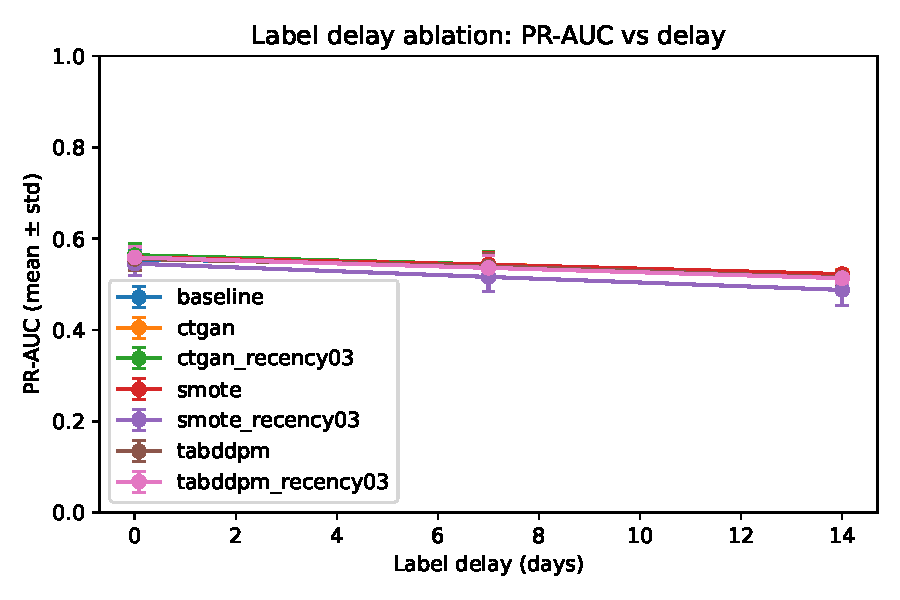
\includegraphics[width=0.95\linewidth]{figures/label_delay_ablation.pdf}
\caption{PR-AUC sensitivity to label delay.}
\end{figure}

\subsection{4.8 Sliding vs. static training (supplementary)}

Five splits; mean PR-AUC ~0.583 (static) vs ~0.570 (sliding) (\texttt{results/sliding_window/results.csv}).

\begin{figure}[t]
\centering
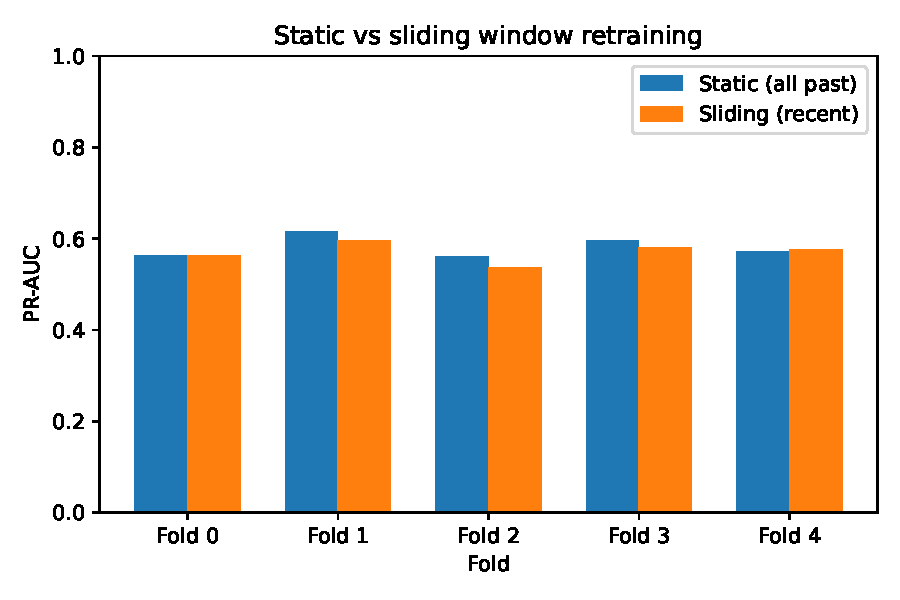
\includegraphics[width=0.95\linewidth]{figures/sliding_window_comparison.pdf}
\caption{static vs. sliding retraining.}
\end{figure}

\subsection{4.9 Synthetic-sample fidelity diagnostics (supplementary)}

To address sample-quality concerns for CTGAN and TabDDPM, we run a lightweight fidelity audit on synthetic positives across the same 4 temporal folds (\texttt{src/run_fidelity_analysis.py}). For tractability, this uses target rate 10\%, max 5000 synthetic positives/fold, and reduced generator budgets (CTGAN epochs=3, TabDDPM epochs=2, timesteps=50). We report numeric quantile L1 (lower is better), categorical TV distance (lower is better), correlation MAD on numeric features (lower is better), and real-vs-synthetic AUC from a discriminator (closer to 0.5 is better).

\begin{table}[t]
\centering
\caption{Supplementary fidelity diagnostics (mean across folds).}
\begin{tabular}{ccccc}
\toprule
Method & Num quantile L1 $\downarrow$ & Cat TV $\downarrow$ & Corr MAD $\downarrow$ & Real-vs-synth AUC \\
\midrule
CTGAN & 9,829.68 & 0.145 & 0.112 & 1.000 \\
TabDDPM & 18,916,262.15 & 1.000 & 0.118 & 1.000 \\
\bottomrule
\end{tabular}
\end{table}

These diagnostics indicate low distribution fidelity in this lightweight setting, especially for TabDDPM on mixed-type features. This helps explain why downstream gains remain inconsistent and why we treat generative results as protocol-dependent rather than universally reliable.


\section{5. Analysis}

\subsection{5.1 Why low-power results matter}

The paired tests in §4.4 do not reach α = 0.05, despite moderate mean PR-AUC deltas versus the baseline. Under temporal evaluation, that is still informative: it characterizes what generic SMOTE, CTGAN, and TabDDPM pipelines achieve on a standard benchmark when leakage is controlled. Importantly, fold-level \textbf{n = 4} gives these tests limited power, so we treat p-values as weak evidence and emphasize effect sizes, fold variability, and protocol realism.

\subsection{5.2 Fold heterogeneity}

Rankings move by fold (§4.3) because validation regimes differ and training grows in the expanding window. Oversampling perturbs training only; it cannot stabilize rankings across shifts.

\subsection{5.3 Generators, drift, and drift-dependent effects}

Domain AUC spans roughly 0.82--0.92 (§4.3). Because our drift metric is correlated with fold difficulty, the correlation sign depends on how “effect” is defined; in our tables we report deltas relative to the baseline, so negative r values (\textbf{n = 4}) are exploratory and best read as: \textbf{higher drift is associated with larger absolute augmentation effects} (often benefits in this run), not as a stable causal relationship. A plausible hypothesis remains that generators fit the training fraud distribution; under covariate shift, synthetic points can either improve coverage or amplify mismatch depending on how fraud modes evolve. SMOTE interpolates between real points; GANs and diffusion sample new points—different failure modes.

\subsection{5.4 Recency}

Recency restricts positives to the latest \textbf{30%}. Under temporal evaluation, this creates an asymmetry: \textbf{CTGAN-recency} and \textbf{TabDDPM-recency} remain close to their non-recency variants (mean PR-AUC \(\approx 0.569\) and \(\approx 0.564\)), whereas \textbf{SMOTE-recency} drops noticeably (mean PR-AUC \(\approx 0.552\)). In §4.6, SMOTE-recency is therefore \textbf{neutral overall} (though it hurts in some folds). A plausible reading is that thinning positives reduces minority coverage for interpolation-based SMOTE more severely than it damages the generators’ learned mapping.

\subsection{5.5 Label delay}

Delay removes labeled training rows before validation (§3.1). Oversampling cannot recover features from transactions that were never in training; the parallel decline across methods in §4.7 matches that story.

\subsection{5.6 Selection on validation}

Choosing the best target fraud rate per fold and method on validation PR-AUC can be optimistic relative to a fixed rate chosen a priori. Mitigations: an inner temporal split for rate selection, or reporting a fixed 5% configuration—see §3.3.

\subsection{5.7 Why fidelity checks matter}

The supplementary fidelity audit (§4.9) gives a useful mechanistic signal: synthetic samples are easy to distinguish from real frauds (real-vs-synth AUC \(\approx\) 1.0 for both CTGAN and TabDDPM in that run), and TabDDPM shows especially weak categorical fidelity there. This does not invalidate the downstream benchmark results, but it clarifies why augmentation effects can be unstable: utility can improve in some folds even when synthetic realism is imperfect, and weak fidelity can cap generalization under shift.


\section{6. Discussion}

\subsection{6.1 Synthesis}

Sections 4--5 give results and analysis; we do not repeat them here. In short: on IEEE-CIS under our protocol, generative oversampling shows moderate average gains over the baseline, but these gains are not statistically significant with four folds (n=4); recency and label-delay behavior follow §5; drift--performance links are hypothesis-generating.

\subsection{6.2 Practical implications for practitioners}

\begin{itemize}
\item \textbf{Generators are optional, not default.} CTGAN and TabDDPM require substantially more training iterations and operational effort than SMOTE; in our study they show moderate mean PR-AUC gains over baseline but no statistically significant baseline improvements with n=4 folds. The extra overhead is hard to justify unless it works in your temporally split validation.
\item \textbf{Start with simpler tools (and a good protocol).} A leakage-safe temporal validation scheme and a well-tuned tree model on real data already go a long way; SMOTE (or a careful variant) is a sensible first step before deploying heavy generative models.
\item \textbf{Monitor drift explicitly.} When train--test drift is high, augmentation effects are more variable and can flip sign; monitoring domain-shift signals can guide when to trust augmentation.
\item \textbf{Treat synthetic oversampling as a surgical tool, not a default.} Prefer it for clearly identified pain points, and account for privacy/compliance considerations in regulated settings.

\end{itemize}
\subsection{6.3 Ethical considerations (for AIES-style review)}

Because synthetic data can be a privacy-adjacent artifact and can change what downstream models learn from rare events, ethical implications deserve explicit attention even in a performance-focused evaluation. We do not study demographic fairness directly, nor do we quantify how synthetic fraud impacts bias in protected attributes; however, practitioners should treat synthetic augmentation as a potential risk factor for amplifying dataset-specific correlations that correlate with sensitive groups. In addition, fraud detection systems operate under asymmetric costs: false negatives typically have immediate financial and customer impact, while false positives create operational burden and customer friction. Our results suggest that oversampling---especially deep generation---should be deployed only when it yields \textbf{clear} and \textbf{temporally robust} gains under leakage-safe protocols, since uncontrolled augmentation could otherwise increase harm.

\subsection{6.4 Limitations}

\begin{itemize}
\item \textbf{Single primary dataset.} Results on IEEE-CIS may not transfer to other fraud portfolios.
\item \textbf{Tabular, transaction-level view only.} Work is limited to engineered tabular representations.
\item \textbf{Limited folds.} We use four temporal folds; this bounds statistical power and makes paired p-values less informative for small effects. Drift correlations are exploratory.
\item \textbf{Lightweight fidelity diagnostics.} We added supplementary distribution-fidelity checks for synthetic positives, but they are coarse and use reduced generator budgets for tractability; stronger, fully tuned fidelity evaluation remains future work.
\item \textbf{Restricted label-delay and recency settings.} We evaluate 7- and 14-day delays and a 30% recency fraction.
\item \textbf{No explicit adversary modeling or privacy analysis.} These are important for deployment, but orthogonal to the oversampling-under-shift question.

\end{itemize}
\subsection{6.5 Directions for future work}

\begin{itemize}
\item Multi-dataset temporal evaluation and richer shift regimes.
\item Structure-aware generators (sequence/graph) under the same temporal protocol.
\item More realistic label-delay regimes.
\item Targeted augmentation for rare typologies.


\end{itemize}
\section{7. Conclusion}

We study when synthetic oversampling improves or degrades rare-event fraud detection under leakage-safe temporal evaluation on the IEEE-CIS benchmark. Across four temporal folds, deep generative oversampling (CTGAN, TabDDPM) yields moderate average gains over the class-weighted baseline but does not show statistically significant improvements under our paired tests (n=4). SMOTE remains a competitive and simple alternative, and recency-aware synthesis shows limited or mixed benefit: CTGAN/TabDDPM recency helps within our protocol, while SMOTE-recency is neutral overall but harms in some folds.

To explain these patterns, we relate oversampling impact to train--validation drift using a domain-classifier signal: generator performance is more consistent with drift-dependent effects (exploratory with four folds). Finally, under a label-delay protocol, oversampling does not recover the performance lost when recent labeled training data are withheld.

Overall, our results suggest that practitioners should treat synthetic oversampling—especially deep tabular generators—as an evidence-driven option rather than a default remedy for imbalance. We recommend that fraud-detection studies report performance under time-respecting protocols and label-delay regimes before claiming benefits from sophisticated synthetic-data generators.



\begin{thebibliography}{8}
\bibitem{ref1} N. V. Chawla, K. W. Bowyer, L. O. Hall, and W. P. Kegelmeyer. SMOTE: Synthetic Minority Over-sampling Technique. \emph{Journal of Artificial Intelligence Research}, 16:321--357, 2002.
\bibitem{ref2} L. Xu, M. Skoularidou, A. Cuesta-Infante, and K. Veeramachaneni. Modeling Tabular Data using Conditional GAN. In \emph{Advances in Neural Information Processing Systems 32 (NeurIPS 2019)}. (Introduces CTGAN and TVAE, a VAE adapted for tabular data.)
\bibitem{ref3} A. Kotelnikov, D. Baranchuk, I. Rubachev, and A. Babenko. TabDDPM: Modelling Tabular Data with Diffusion Models. In \emph{Proceedings of the 40th International Conference on Machine Learning (ICML 2023)}, Vol. 202, pp. 17564--17579.
\bibitem{ref4} IEEE-CIS Fraud Detection. Kaggle competition dataset, 2019. \url{https://www.kaggle.com/c/ieee-fraud-detection}
\bibitem{ref5} A. Dal Pozzolo, O. Caelen, R. A. Johnson, and G. Bontempi. Calibrating Probability with Undersampling for Unbalanced Classification. In \emph{2015 IEEE Symposium Series on Computational Intelligence (SSCI)}. IEEE, 2015.
\bibitem{ref6} A. Dal Pozzolo, Y.-A. Le Borgne, O. Caelen, Y. Kessaci, F. Oblé, and G. Bontempi. \emph{Reproducible Machine Learning for Credit Card Fraud Detection - Practical Handbook}. GitHub, 2020. \url{https://github.com/Fraud-Detection-Handbook/fraud-detection-handbook}
\bibitem{ref7} S. Rabanser, S. Günnemann, and Z. C. Lipton. Failing Loudly: An Empirical Study of Methods for Detecting Dataset Shift. In \emph{Advances in Neural Information Processing Systems 32 (NeurIPS 2019)}.
\bibitem{ref8} H. He and E. A. Garcia. Learning from Imbalanced Data. \emph{IEEE Transactions on Knowledge and Data Engineering}, 21(9):1263--1284, 2009.
\end{thebibliography}
\end{document}